\documentclass[aspectratio=43]{beamer}
\usepackage[latin1]{inputenc}
\usepackage{amsmath}
\usepackage{amsfonts}
\usepackage{amssymb}
\usepackage{makeidx}
\usepackage{graphicx}
\usepackage{array}

% Customization
\mode<presentation>{
	\usetheme{CambridgeUS}
	\usecolortheme{dolphin}
	\setbeamertemplate{navigation symbols}{}
}

% Define colors
\definecolor{darkgreen}{rgb}{0.0, 0.5, 0.13}
\definecolor{darkblue}{rgb}{0.0, 0.0, 0.55}
\definecolor{darkred}{rgb}{0.55, 0.0, 0.0}

% Title and author
\title[Perturbative QCD predictions for Higgs production]{pQCD predictions for Higgs production}
\author{\textbf {Jes\'us Urtasun Elizari}}
%\institute{\textbf {University of Milan}}
\date{Milan, February 2021}

\begin{document}

% Front slide
\begin{frame}

	%\maketitle
	\vspace{1.0 cm}
	
	\center{\color{blue}High precision perturbative QCD predictions \\ for LHC physics}
	
	\vspace{0.25 cm}
	\center{Jes\'us Urtasun Elizari}
	\center{Milan, February 2021}

	\begin{figure}
		\minipage{1\textwidth}
		
\includegraphics[width = 3.0 cm]{plots/unimi.png}
		\hfill
		
\includegraphics[width = 3.0 cm]{plots/n3pdf.png}
		\hfill
		
\includegraphics[width = 3.0 cm]{plots/erc.png}
		\endminipage
	\end{figure}

	\vspace{1.0 cm}
	
	{\scriptsize \color{blue} This project has received funding from the European Union$'$s Horizon 2020 research and innovation program under grant agreement No 740006.}

\end{frame}

% Introduction
\begin{frame}

	\frametitle{Outline}
	
	\begin{enumerate}
		\item {\color{blue}QCD factorization in a nutshell}
		\begin{itemize}
			\item QCD factorization
			\item PDFs and partonic cross section
		\end{itemize}
		\item {\color{blue}The N3PDF project}
		\begin{itemize}	
			\item Machine Learning for PDFs
		\end{itemize}	
		\item {\color{blue}Fast predictions for resummed distributions}
		\begin{itemize}
			\item Higher order corrections
			\item All order resummation
			\item \textbf{HTurbo} numerical code
		\end{itemize}
		\item {\color{blue}Conclusions}
	\end{enumerate}
	
\end{frame}

% QCD in a nutshell
\begin{frame}

	\center{\color{blue}QCD factorization in a nutshell}

\end{frame}

% Factorization theorem
\begin{frame}

	\frametitle{QCD factorization in a nutshell}
	\framesubtitle{Factorization theorem}

	\center \footnotesize $h_{1}(p_{1}) + h_{2}(p_{2}) \rightarrow F + X$ 
	
	\begin{figure}
		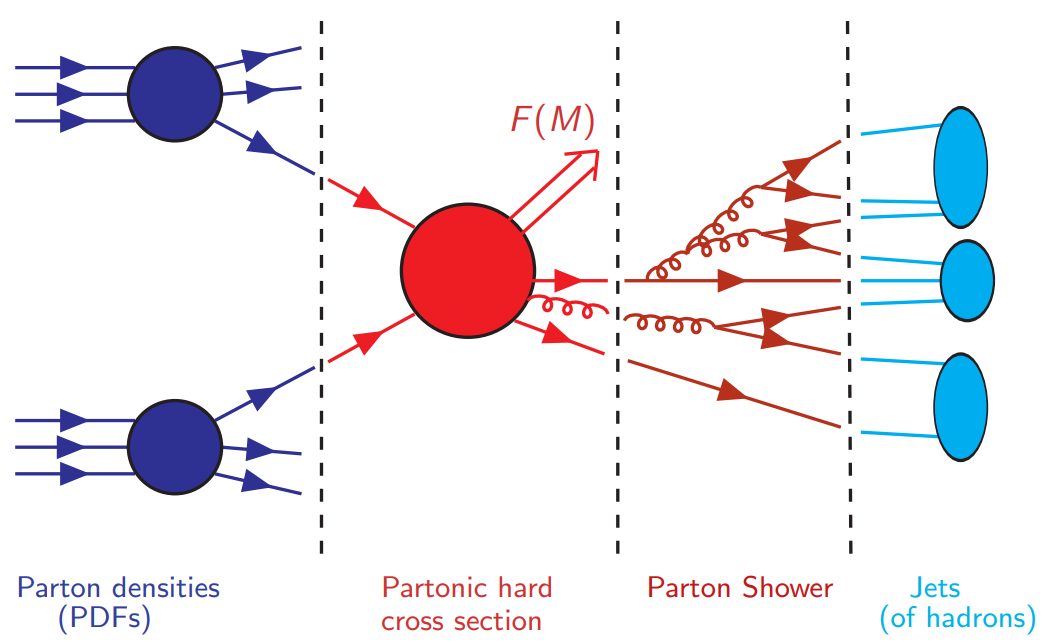
\includegraphics[width = 7 cm]{plots/section1/factorization_1.png}
	\end{figure}
	
	\center \footnotesize {Factorize process as {\color{blue}PDFs} and {\color{red} partonic (hard) interaction}	
	\begin{equation}
		\sigma^{\textrm{F}}(p_{1}, p_{2}) = \sum_{\alpha, \beta}
		\int_{0}^{1} dx_{1} dx_{2} \; {\color{blue} f_{\alpha/h_{1}}(x_{1}, \mu_{F}^{2}) \ast f_{\beta/h_{2}}(x_{2}, \mu_{F}^{2})}
		\; \ast \;  
		{\color{red}\hat{\sigma}^{\textrm{F}}_{\alpha \beta}(x_{1}p_{1}, x_{2}p_{2}, \alpha_{s}(\mu_{R}^{2}), \mu_{F}^{2})} \nonumber
	\end{equation}}
\end{frame}

% Perturbative QCD
\begin{frame}

	\frametitle{QCD factorization in a nutshell}
	\framesubtitle{Perturbative QCD}
	
	\footnotesize Accurate QCD predictions require precise knowledge of {\color{blue}PDFs} and {\color{red} partonic cross section}
	\begin{columns}
		
		\column{0.45\textwidth}
		
		\begin{itemize}
			\item \footnotesize Born cross section is the leading-order (LO) term of the perturbative series
			\item \footnotesize $\sigma^{(1)}, \sigma^{(2)}, \sigma^{(3)}$ are the NLO, NNLO, N$^{3}$LO corrections
		\end{itemize}
		
		\column{0.45\textwidth}
		\begin{figure}[!htb]
			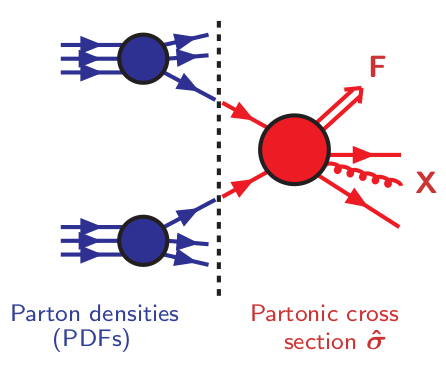
\includegraphics[width = 4 cm]{plots/section1/factorization_3.png}
		\end{figure}
	
	\end{columns}

	\vspace{0.5cm}	
	
	\begin{equation}
		\hat{\sigma} = \sigma^{\texttt{Born}} \Big( 1 +
		\alpha_{s} \sigma^{(1)} + 
		\alpha_{s}^{2} \sigma^{(2)} + 
		\alpha_{s}^{3} \sigma^{(3)} + ... \Big) \nonumber
	\end{equation}
	
	\footnotesize LO predictions strongly depend on unphysical renormalization and factorization scales \\
	{\color{red}Need higher order corrections to increase theoretical accuracy!}

\end{frame}

% The N3PDF project
\begin{frame}

	\center{\color{blue}The N3PDF project}

\end{frame}

% General structure of a fit
\begin{frame}
	
	\frametitle{The N3PDF project}
	\framesubtitle{General structure of n3fit}

	\footnotesize Parton Distribution Functions (PDFs) can not be predicted or measured\\
	{\color{red} PDFs need to be extracted from data!}

	\vspace{0.5cm}
	
	\begin{columns}
		
		\column{0.5\textwidth}
		
		
\includegraphics[width = 1.5cm]{plots/section2/TF.png}
				
		\column{0.5\textwidth}
				
		
\includegraphics[width = 2.5cm]{plots/section2/Keras.png}
		
	\end{columns}
	
	\vspace{0.5cm}
	
	\begin{itemize}
		\item \footnotesize Use TensorFlow and Keras to determine the PDFs
		\item \footnotesize Use Stochastic Gradient Descent {\color{violet} n3fit} replacing primitive genetic algorithms
	    \item \footnotesize See paper by S.Carraza - J.Cruz-Martinez \\
		\footnotesize {\color{blue}"Towards a new generation of parton densities with deep learning models",\\ https://arxiv.org/abs/1907.05075}
	\end{itemize}

\end{frame}

% The N3PDF project
\begin{frame}

	\frametitle{The N3PDF project}
	\framesubtitle{Operator implementation in TF}
	
	\begin{figure}
		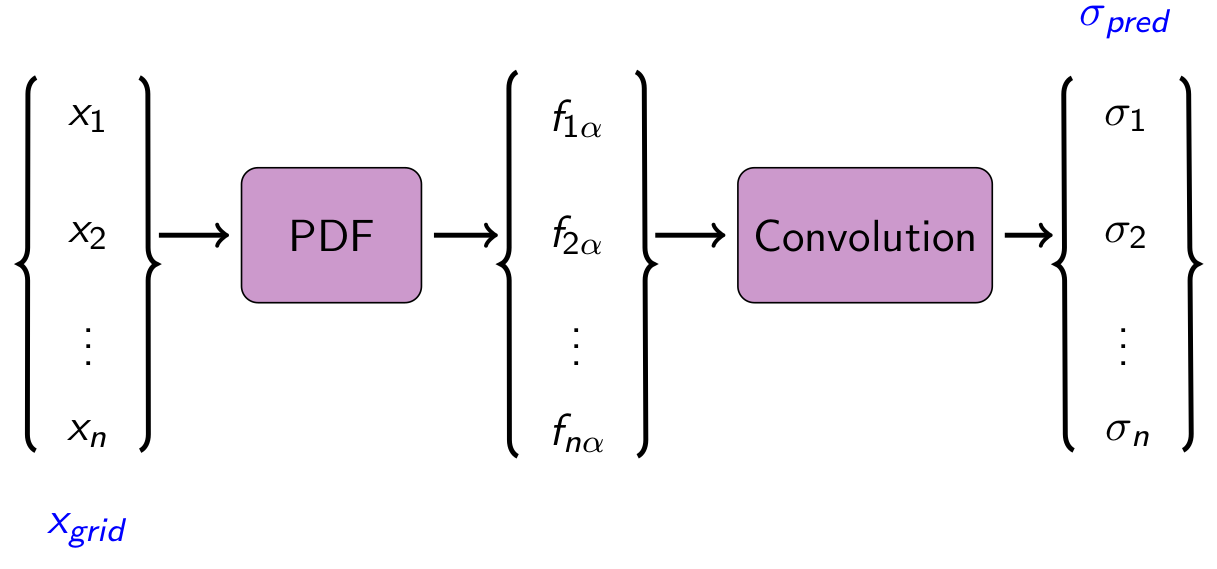
\includegraphics[width = 8.5 cm]{plots/section2/TF_convolution.png}
	\end{figure}


	\begin{itemize}
		\item \footnotesize Build a NN model to compute $\sigma_{pred}$ observables from a grid $x_{i}$
		\item \footnotesize Perform $\chi^{2}$ minimization comparing with data
		\item \footnotesize Update values of PDF $\longrightarrow$ {\color{violet} Fit}
	\end{itemize}

\end{frame}

% The N3PDF project
\begin{frame}

	\frametitle{The N3PDF project}
	\framesubtitle{Operator implementation in TF}
		
	\begin{figure}
		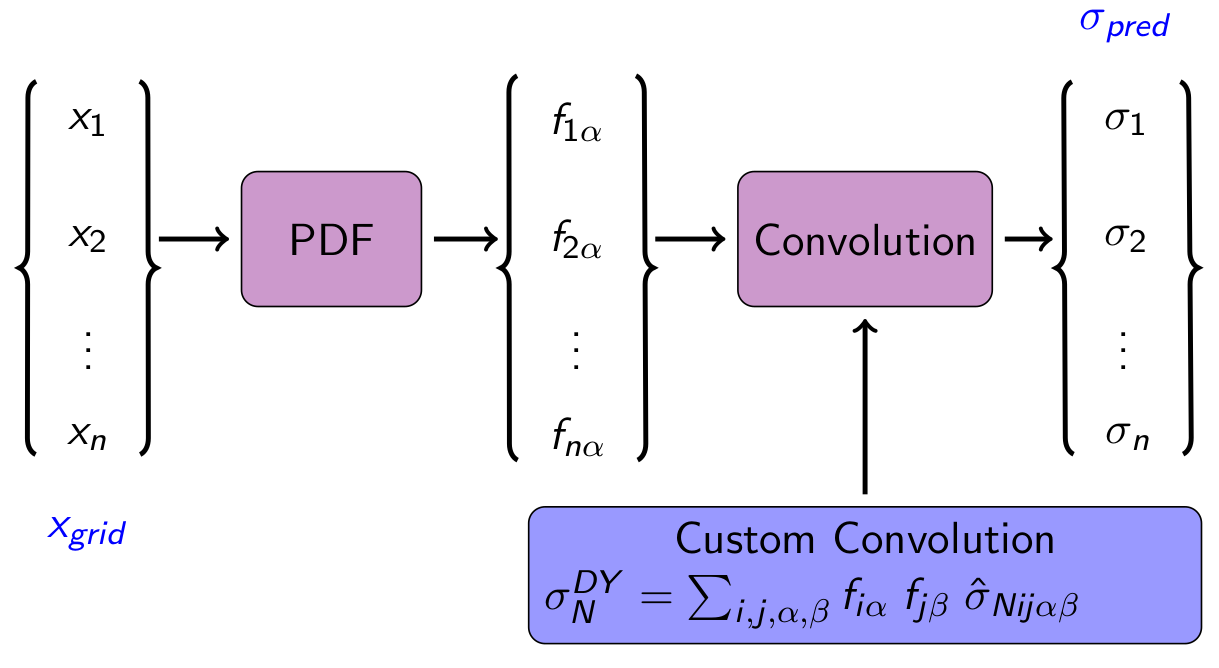
\includegraphics[width = 8.5 cm]{plots/section2/TF_convolution2.png}
	\end{figure}

	\begin{enumerate}
		\item \footnotesize TF relies in symbolic computation $\longrightarrow$ High memory usage
		\item \footnotesize Implement c++ operator replacing the convolution
		\item Further details in Urtasun-Elizari et al.\\
		{\color{blue}"Towards hardware acceleration for parton densities estimation",\\ https://arxiv.org/abs/1909.10547}
	\end{enumerate}

\end{frame}

% HTurbo
\begin{frame}

\center{\color{blue}HTurbo: Fast predictions for resummed distributions}

\end{frame}

% HTurbo II - qT resummation
\begin{frame}

	\frametitle{HTurbo}
	\framesubtitle{All order $q_{\perp}$ resummation}
	
	\begin{columns}
	
		\column{0.55\textwidth}
		
		\center	\footnotesize Study the differential $q_{\perp}$ distribution \\
		\center	$h_{1}(p_{1}) + h_{2}(p_{2}) \longrightarrow F(M, {\color{red}q_{\perp}}) + X$
	
		\column{0.45\textwidth}
		
		\begin{figure}
			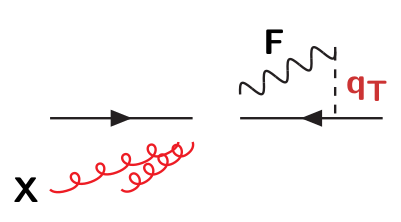
\includegraphics[width = 3.5cm]{plots/qT_diagram.png}
		\end{figure}

	\end{columns}

	\footnotesize {$$\int_{0}^{Q_{\perp}^{2}} \; dq_{\perp}^{2} \frac{d\hat{\sigma}}{dq_{\perp}^{2}} \sim c_{0} + \alpha_{s}(c_{12}L^{2} + c_{11}L + c_{10}) + ..., \textrm{\quad being \quad} L = \ln (q_{\perp} / M^{2})$$}

	\begin{figure}
		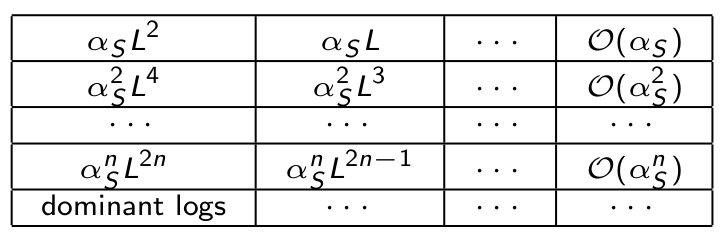
\includegraphics[width = 7cm]{plots/qT_logs_table.png}
	\end{figure}

	\footnotesize Truncated fixed order predictions lead to {\color{red} logarithmic enhancement $\alpha_{s}^{n}\ln^{m}(M^{2}/q_{\perp}^{2})$} \\
	\center \footnotesize {\color{red} All order resummation is needed} \\

\end{frame}

% HTurbo IV - DYturbo
\begin{frame}

	\frametitle{HTurbo}
	\framesubtitle{Starting point: DYTurbo}

	\footnotesize $q_{\perp}$ resummation implemented in numerical codes \textbf{HqT} and \textbf{HRes} {\color{blue}[Catani et al.]} \\
	\footnotesize Higher order accuracy require {\color{red}high computation times}
	
	\vspace{0.5cm}

	\footnotesize Numerical code \textbf{DYTurbo} {\color{blue}[Camarda et al. ATLAS collaboration, {\color{blue} \href{https://arxiv.org/abs/1910.07049}{1910.07049}}]},\\
	fast and precise $q_{\perp}$ resummation and several improvements for Drell-Yan ($h_{1} + h_{2} \rightarrow V + X \rightarrow l^{+}l^{-} + X$)

	\begin{itemize}
		\item \footnotesize {\color{red}Goal}: set up a numerical code generalizing  \textbf{DYTurbo} for Higgs boson production
		\item \footnotesize {\color{red}Goal}: extend theoretical accuracy up to N$^{3}$LL+N$^{3}$LO and to other processes
	\end{itemize}

	\vspace{0.5cm}
	
	\footnotesize Numerical code \textbf{HTurbo} {\color{blue}[Ferrera, Urtasun-Elizari (in preparation)]} \\
	Fast and precise $q_{\perp}$ resummation and for Higgs boson production
	\begin{itemize}
		\item \footnotesize Old versions as \textbf{HqT} and \textbf{HRes} in Fortran
		\item \footnotesize c++ allows for optimization in the integration routines
	\end{itemize}

\end{frame}

% Results LL
\begin{frame}
	
	\frametitle{Results}
	\framesubtitle{Comparison with HRes and HqT - LL}
	
	\begin{figure}
		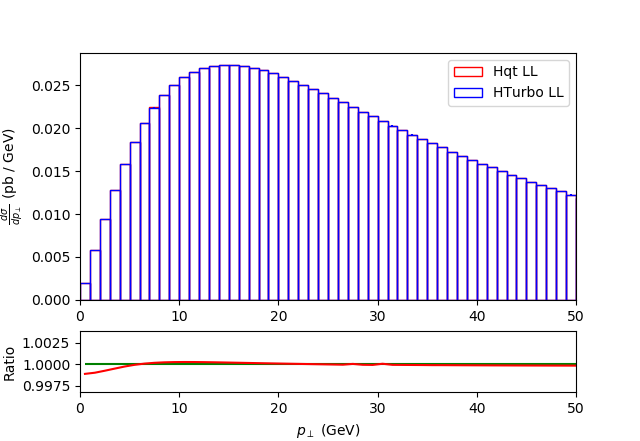
\includegraphics[width = 8cm]{plots/hturbo_LL.png}
	\end{figure}
	
	\begin{itemize}
		\item \footnotesize HTurbo $q_{\perp}$ distribution vs HRes and HqT at LL
		\item \footnotesize Excellent numerical agreement up to the $0.1\%$ level {\color{darkgreen}$\checkmark$} 
	\end{itemize}

\end{frame}

% Results NLL
\begin{frame}

	\frametitle{Results}
	\framesubtitle{Comparison with HTurbo and HqT - NLL}
	
	\begin{figure}
		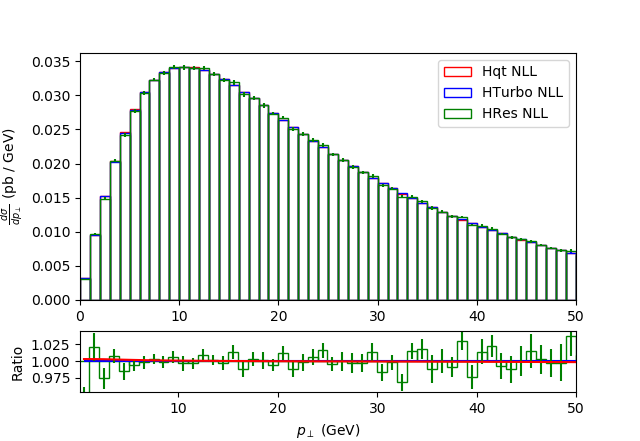
\includegraphics[width = 8cm]{plots/hturbo_NLL.png}
	\end{figure}
	
	\begin{itemize}
		\item \footnotesize HTurbo $q_{\perp}$ distribution vs HRes and HqT at NLL
		\item \footnotesize Excellent numerical agreement up to the $0.1\%$ level {\color{darkgreen}$\checkmark$} 
	\end{itemize}

\end{frame}

% Results NNLL
\begin{frame}

	\frametitle{Results}
	\framesubtitle{Comparison with HRes and HqT - NNLL}
	
	\begin{figure}
		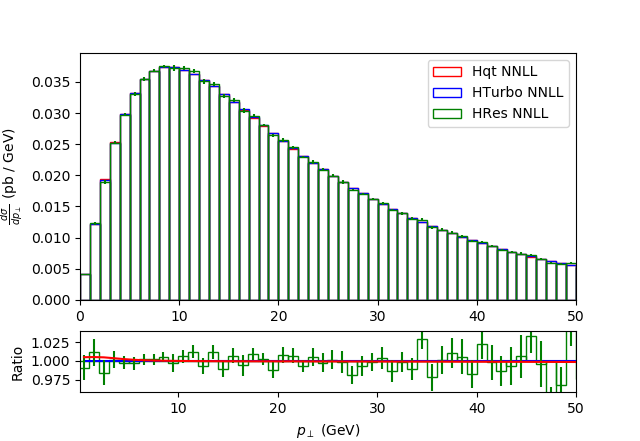
\includegraphics[width = 8cm]{plots/hturbo_NNLL.png}
	\end{figure}
	
	\begin{itemize}
		\item \footnotesize HTurbo $q_{\perp}$ distribution vs HRes and HqT at NNLL
		\item \footnotesize Excellent numerical agreement up to the $0.1\%$ level {\color{darkgreen}$\checkmark$} 
\end{itemize}

\end{frame}

% Results all
\begin{frame}
	
	\frametitle{Results}
	\framesubtitle{Comparison HRes and HqT - all orders}
	
	\begin{figure}
		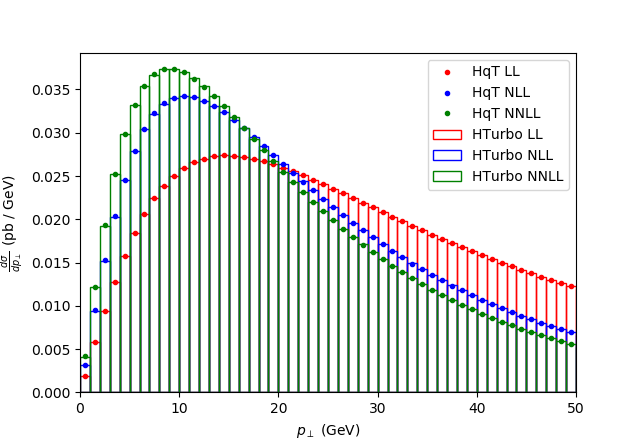
\includegraphics[width = 8cm]{plots/hturbo_all_orders.png}
	\end{figure}
	
	\begin{itemize}
		\item \footnotesize Higher orders lead to more accurate predictions {\color{darkgreen}$\checkmark$} 
		\item \footnotesize \textbf{HRes} needs 3 days to produce NNLL distribution $\rightarrow$ {\color{blue} 3 minutes with \textbf{HTurbo}!} {\color{darkgreen}$\checkmark$} 
		\item \footnotesize Agreement up to NNLL $\longrightarrow$ {\color{blue}ready for N$^{3}$LL}
	\end{itemize}

\end{frame}

% Conclusions
\begin{frame}
	
	\frametitle{Summary $\&$ Conclusions}

	\vspace{2.0 cm}
	
	\begin{enumerate}
		\item \footnotesize Precise knowledge of PDFs and partonic cross sections are required towards the precision era of the LHC
		\item \footnotesize Machine Learning models provide a robust way for PDFs determination optimized through {\color{blue}operator implementation in TF}
		\item \footnotesize We develop a numerical code \textbf{HTurbo}, implementing $q_{\perp}$ resummation for Higgs boson production, which is {\color{blue} faster than any of the existing codes}
		\item \footnotesize Next steps: 
		\begin{itemize}
			\item \footnotesize Validate results at NNLO
			\item \footnotesize Include full {\color{blue}N$^{3}$LO} prediction
			\item \footnotesize Perform phenomenological studies comparing with LHC data
		\end{itemize}

	\end{enumerate}

	\vspace{2.0 cm}

\end{frame}

% Conclusions
\begin{frame}

	\center {\color{blue}Thank you!}

	\begin{figure}
		
\includegraphics[width = 2.5 cm]{plots/thinking.png}
	\end{figure}		

	{\footnotesize \color{blue} This project has received funding from the European Union$'$s Horizon 2020 research and innovation program under grant agreement No 740006.}

\end{frame}

\end{document}